\section{Auswertung}
Die zu Beginn des Versuchs durchgeführte Nullmessung ergibt die in Abb.\ref{Leermessung1} dargestellte Energieverteilung. Sie zeigt deutlich den bei $^{137}$Cs auftretenden Peak um $662 \, \si{\kilo\electronvolt}$ sowie die davor liegende
Compton-Kante. Es wurden $11059$ Ereignisse in $60.42 \, \si{\second}$, oder $183 \,  \pm \, 3\, \frac{\text{counts}}{\si{\second}}$ gemessen.
Die in den Spektren gezeigten Fehlerbalken stammen von den, durch die Poisson-Verteilung gegebenen, $\sqrt{n}$ Fehler.
\begin{figure}[H]
  \centering
  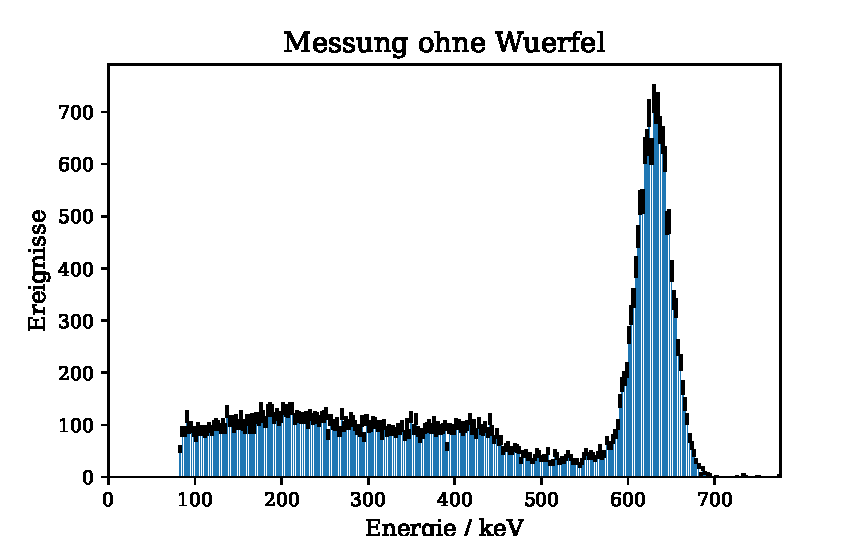
\includegraphics{plots/leer.pdf}
  \caption{Schematische Darstellung des Versuchsaufbaus.\cite{anleitung}}
  \label{Leermessung1}
\end{figure}
\subsection{Leerer Würfel}
Die Untersuchungen des leeren Würfels ergeben die in den Abb.4 Abb.5 gezeigten Spektren. Der Intensitätsvektor
für die verschiedenen Projektionen der ersten Messung ist in (7) zu finden, die der zweiten in (8).
Aufgrund des homogenen Aufbaus des Würfels,
werden für nicht vermessene Projektionsrichtungen die Werte von äquivalenten Projektionen eingesetzt.
Vermessen wurden die Projektionsrichtungen 1, 3, 13, 14, 15

\begin{equation}
	\vec{I_1}=
	\begin{pmatrix}
		\num{180.1 \pm 2.4} \\
		\num{180.1 \pm 2.4} \\
		\num{180.1\pm 2.4} \\
		\num{178.8\pm 2.4} \\
		\num{178.8\pm 2.4} \\
		\num{178.8\pm 2.4} \\
		\num{176.6\pm 2.4} \\
		\num{177.0\pm 2.4} \\
		\num{175.9\pm 2.4} \\
    \num{176.6\pm 2.4} \\
    \num{177.0\pm 2.4} \\
    \num{175.9\pm 2.4} \\
	\end{pmatrix}
    \sfrac{\text{counts}}{\text{s}}
	\label{eq:vecleer1}
\end{equation}
\begin{equation}
	\vec{I_2}=
	\begin{pmatrix}
		\num{171.7 \pm 2.5} \\
		\num{171.7 \pm 2.5} \\
		\num{171.7\pm 2.5} \\
		\num{173.3\pm 2.4} \\
		\num{173.3\pm 2.4} \\
		\num{173.3\pm 2.4} \\
		\num{165.2\pm 2.5} \\
		\num{161.8\pm 2.5} \\
		\num{174.1\pm 1.9} \\
    \num{165.2\pm 2.5} \\
    \num{162.8\pm 2.5} \\
    \num{174.1\pm 1.9} \\
	\end{pmatrix}
    \sfrac{\text{counts}}{\text{s}}
	\label{eq:vecleer2}
\end{equation}
\begin{figure}[H]
  \centering
  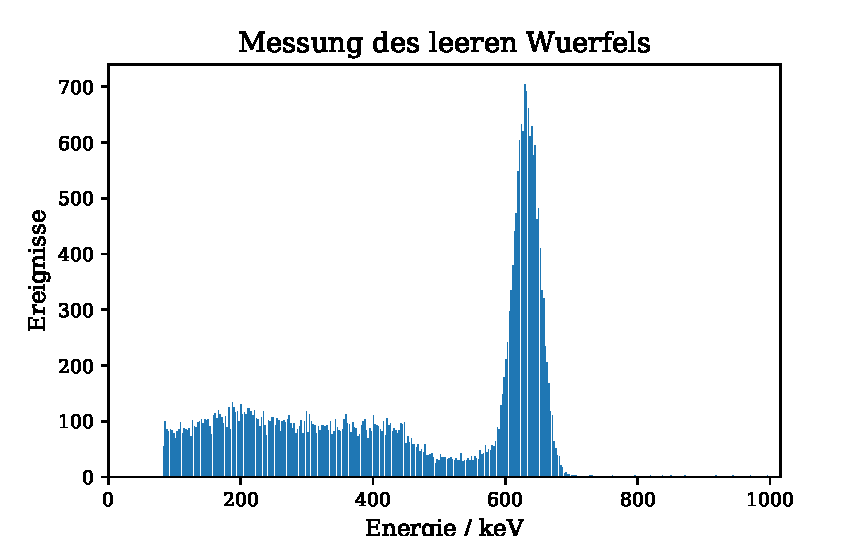
\includegraphics{plots/Alu_leer.pdf}
  \caption{Spektrum des leeren Würfels (1. Messung).\cite{anleitung}}
  \label{Leermessung}
\end{figure}
\begin{figure}[H]
  \centering
  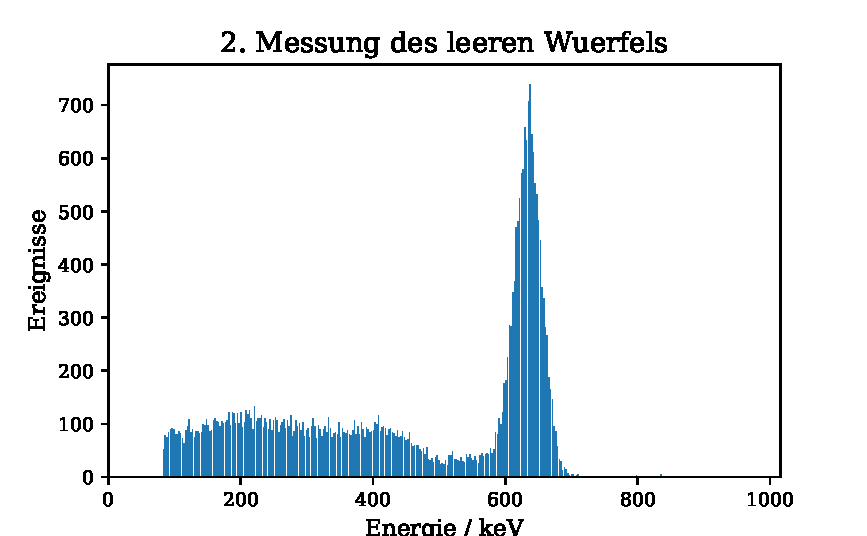
\includegraphics{plots/Alu_leer2.pdf}
  \caption{Spektrum des leeren Würfels (2. Messung).\cite{anleitung}}
  \label{Leermessung}
\end{figure}
\subsection{Untersuchung der Würfel 2 und 3}
Die Bestimmung des Absorptionskoeffizienten der Würfel 2 und 3, welche jeweils komplett aus Aluminium oder Blei bestehen, nutzt die Tatsache, dass sich durch deren Aufbau die verschiedenen gemessenen Projektionen mitteln lassen
und es möglich ist, die Geometriematrix zu einem Vektor in den einzelnen Komponenten zu summieren. Diese Vektoren $\vec{A_2}$ und $\vec{A_3}$ sind:
\begin{equation}
	\vec{A_2}=
	\begin{pmatrix}
		2\sqrt{2} \\
		3\sqrt{2} \\
		2\sqrt{2} \\
		\sqrt{2}\\
    \sqrt{2}
	\end{pmatrix} \; .
\end{equation}
\begin{equation}
	\vec{A_3}=
	\begin{pmatrix}
		2\sqrt{2} \\
		3\sqrt{2} \\
		2t\sqrt{2} \\
		\sqrt{2}\\
	\end{pmatrix} \; .
\end{equation}
$\vec{A_2}$ und $\vec{A_3}$ erlauben es, mit einen Least-Square-Fit und (6), die Absorptionskoeffizienten zu berechnen. Es ergibt sich:
\begin{equation}
  \text{Würfel 2: } \left(0.22 \pm 0.02\right) \, \frac{1}{\si{\centi\meter}} \nonumber
\end{equation}
\begin{equation}
  \text{Würfel 3: } \left(1.26 \pm 0.09\right) \, \frac{1}{\si{\centi\meter}} \nonumber
\end{equation}
Für Würfel 2 wurden bei der Untersuchung die Projektionsrichtungen 1, 3, 13, 14, 15 und bei Würfel 3: 3, 13, 14, 15
\subsection{Untersuchung von Würfel 5}
Der Würfel unbekannten Aufbaus (Würfel 5) wird mit zwölf Projektionsrichtungen untersucht, um so genauere Schlüsse auf das Material der einzelnen Elementarwürfel zu erlauben. Da der Aufbau des Würfels
gänzlich unbekannt ist, ist es in diesem Fall nicht möglich die Geometriematrix A zu vereinfachen. Der Intensitätsvektor $\vec{I_5}$ und der Logarithmus von $\vec{I_5}$ ($\vec{\tilde{I_5}}$) lauten:
\begin{equation}
	\vec{I_5}=
	\begin{pmatrix}
		\num{35.9 \pm 1.2} \\
		\num{35.3 \pm 1.2} \\
		\num{88.3\pm 1.9} \\
		\num{84.2\pm 1.8} \\
		\num{34.1\pm 1.1} \\
		\num{72.2\pm 1.7} \\
		\num{85.5\pm 1.7} \\
		\num{28.2\pm 1.0} \\
		\num{25.1\pm 1.0} \\
    \num{103.5\pm 1.9} \\
    \num{39.3\pm 1.2} \\
    \num{24.5\pm 0.9} \\
	\end{pmatrix}
    \sfrac{\text{counts}}{\text{s}}
	\label{eq:vec5}
\end{equation}
\begin{equation}
	\vec{I_5}=
	\begin{pmatrix}
		\num{1.6 \pm 0.2} \\
		\num{1.6 \pm 0.2} \\
		\num{0.7\pm 0.1} \\
		\num{0.7\pm 0.1} \\
		\num{1.6\pm 0.2} \\
		\num{0.9\pm 0.1} \\
		\num{0.7\pm 0.1} \\
		\num{1.8\pm 0.2} \\
		\num{1.9\pm 0.2} \\
    \num{0.5\pm 0.1} \\
    \num{1.5\pm 0.2} \\
    \num{2.0\pm 0.2} \\
	\end{pmatrix}
    \sfrac{\text{counts}}{\text{s}}
	\label{eq:vecleer1}
\end{equation}
Die Absorptionskoeffizienten $\mu$ der Teilwürfel lassen sich hiermit wie bei den Würfeln 2 und 3 bestimmen. Es ergibt sich:
\begin{table}[H]
\centering
\caption{Berechnete Absorptionskoeffizienten der einzelnen Teilwürfel.}
\label{companioncube}
\begin{tabular}{c|c|c}
  Elementarwürfel& $\mu$ in $\frac{1}{\si{\second}}$& Zugeordnetes Material \\
  \hline
1 & 0.56 \pm \, 0.09 & Eisen\\
2 & 0.6  \pm \, 0.07&Messing \\
3 & 0.29 \pm\, 0.1  &Aluminium\\
4 & -0.1  \pm\, 0.06&Delrin \\
5 & 0.69 \pm \,0.08 &Messing\\
6 & 0.86  \pm \,0.08& Messing\\
7 & 0.33  \pm \, 0.08& Aluminium\\
8 & 0.49  \pm \,0.07 &Eisen\\
9 & -0.19 \pm \,0.09 &Delrin\\
\end{tabular}
\end{table}
\begin{equation}
	A=
	\begin{pmatrix}
    1& 1& 1& 0& 0& 0& 0& 0& 0\\
    0& 0& 0& 1& 1& 1& 0& 0& 0\\
    0 & 0& 0& 0& 0& 0& 1& 1& 1\\
    1& 0& 0& 1& 0& 0& 1& 0& 0\\
    0& 1& 0& 0& 1& 0& 0& 1& 0\\
    0& 0& 1& 0& 0& 1& 0& 0& 1\\
    0& \sqrt{2}& 0& \sqrt{2}& 0& 0& 0& 0& 0\\
    0& 0& \sqrt{2}& 0&\sqrt{2}& 0& \sqrt{2}& 0& 0\\
    0& 0& 0& 0& 0&\sqrt{2}& 0& \sqrt{2}& 0\\
    0& 0& 0&\sqrt{2}& 0& 0& 0&\sqrt{2}& 0\\
    \sqrt{2}& 0& 0& 0& \sqrt{2}& 0& 0& 0& \sqrt{2}\\
    0& \sqrt{2}& 0& 0& 0& \sqrt{2}& 0& 0& 0
	\end{pmatrix}
\end{equation}
